\chapter[Topic: Loans]{Topic: Loans (10\%-20\%)}

\subsection{Information}

\begin{distributions}[Objective]
The Candidate will understand key concepts concerning loans and how to perform related calculations.
\end{distributions}

\begin{outcomes}[Learning outcomes]
The candidate will be able to:
\begin{enumerate}[label = \alph*)]
	\item	Define and recognize the \textit{definitions} of the following terms:
		\begin{multicols*}{2}
		\begin{itemize}[leftmargin = *]
		\item	Principal;
		\item	Interest;
		\item	Term of loan;
		\item	Outstanding balance;
		\item	Final payment;
			\begin{itemize}
			\item	Drop payment;
			\item	Baloon payment.
			\end{itemize}
		\item	Amortization.
		\end{itemize}
		\end{multicols*}
	\item	Calculate:
		\begin{itemize}[leftmargin = *]
		\item	The missing item given any 4 of :
			\begin{multicols*}{2}
			\begin{itemize}[leftmargin = *]
			\item	Term of loan;
			\item	Interest rate;
			\item	Payment amount;
			\item	Payment period;
			\item	Principal.
			\end{itemize}
			\end{multicols*}
		\item	The outstanding balance at any point in time;
		\item	The amount of interest and principal repayment in a given payment;
		\item	Similar calculations to the above when refinancing is involved.
		\end{itemize}
\end{enumerate}
\end{outcomes}

\begin{ASM_chapter}[Related lessons ASM]
Section 6: Loans
\begin{itemize}
	\item	\nameref{L.-6a}
	\item	\nameref{L.-6b}
	\item	\nameref{L.-6c}
	\item	\nameref{L.-6d}
\end{itemize}
\end{ASM_chapter}

\begin{YTB_vids}[Vidéos YouTube]
\begin{itemize}
	\item	
\end{itemize}
\end{YTB_vids}

\subsection{Résumés des chapitres}

\begin{CHPT_SUMM_AUTO}[label = {L.-6a}]{6a. Amortizing a Loan}
\textbf{Amortization} is reducing the outstanding balance ($B$) of a loan by making payments ($R$) which are part interest ($I$) and part principal ($P$).\\

We're interested in distinguishing the interest and principal portions of each payment for many reasons:
\begin{itemize}[leftmargin = *]
	\item	If you have a mortgage, only the interest portion of the payments are tax deductible. 
	\item	From the lender's point of view, the interest payments are his profit while the principal payments are only returning what he owns.
\end{itemize}

\paragraph{Components of amortizing}
\begin{description}
	\item[$I_{t}$]	\textbf{Interest paid} at the end of year $t$.
	\item[$P_{t}$]	\textbf{Principal repaid} at the end of year $t$.
		\begin{itemize}[leftmargin = *]
		\item	The payments are in geometric progression with a common ratio of $(1 + i)$.\\
				So, $P_{t} = P_{1} (1 + i)^{t - 1}$ for example.
		\end{itemize}
	\item[$R_{t}$]	\textbf{Loan payment} at the end of year $t$.
	\item[$B_{t}$]	\textbf{Outstanding loan} balance at the end of year $t$ (just \textbf{\textit{after}} the loan payment is made).
		\begin{itemize}[leftmargin = *]
		\item	Retrospective method: Looking backwards to the original loan amount, the loan payment and the principal repaid in that payment.
		\item	Prospective method: Looking forward to the remaining payments.\\
				$B_{t} = PV(\text{remaining payments})$
		\end{itemize}
\end{description}

Thus we get:
\begin{align*}
	R_{t}	&= P_{t} + I_{t}	\\
	I_{t}	&= iB_{t - 1}	\\
	B_{t} 	&= B_{t - 1} - P_{t}	\\
	B_{n}	&=	0	&
	B_{0}	&=	L
\end{align*}

An \textbf{amortization schedule} is usually used for organizing the recursive calculation:
\begin{center}
	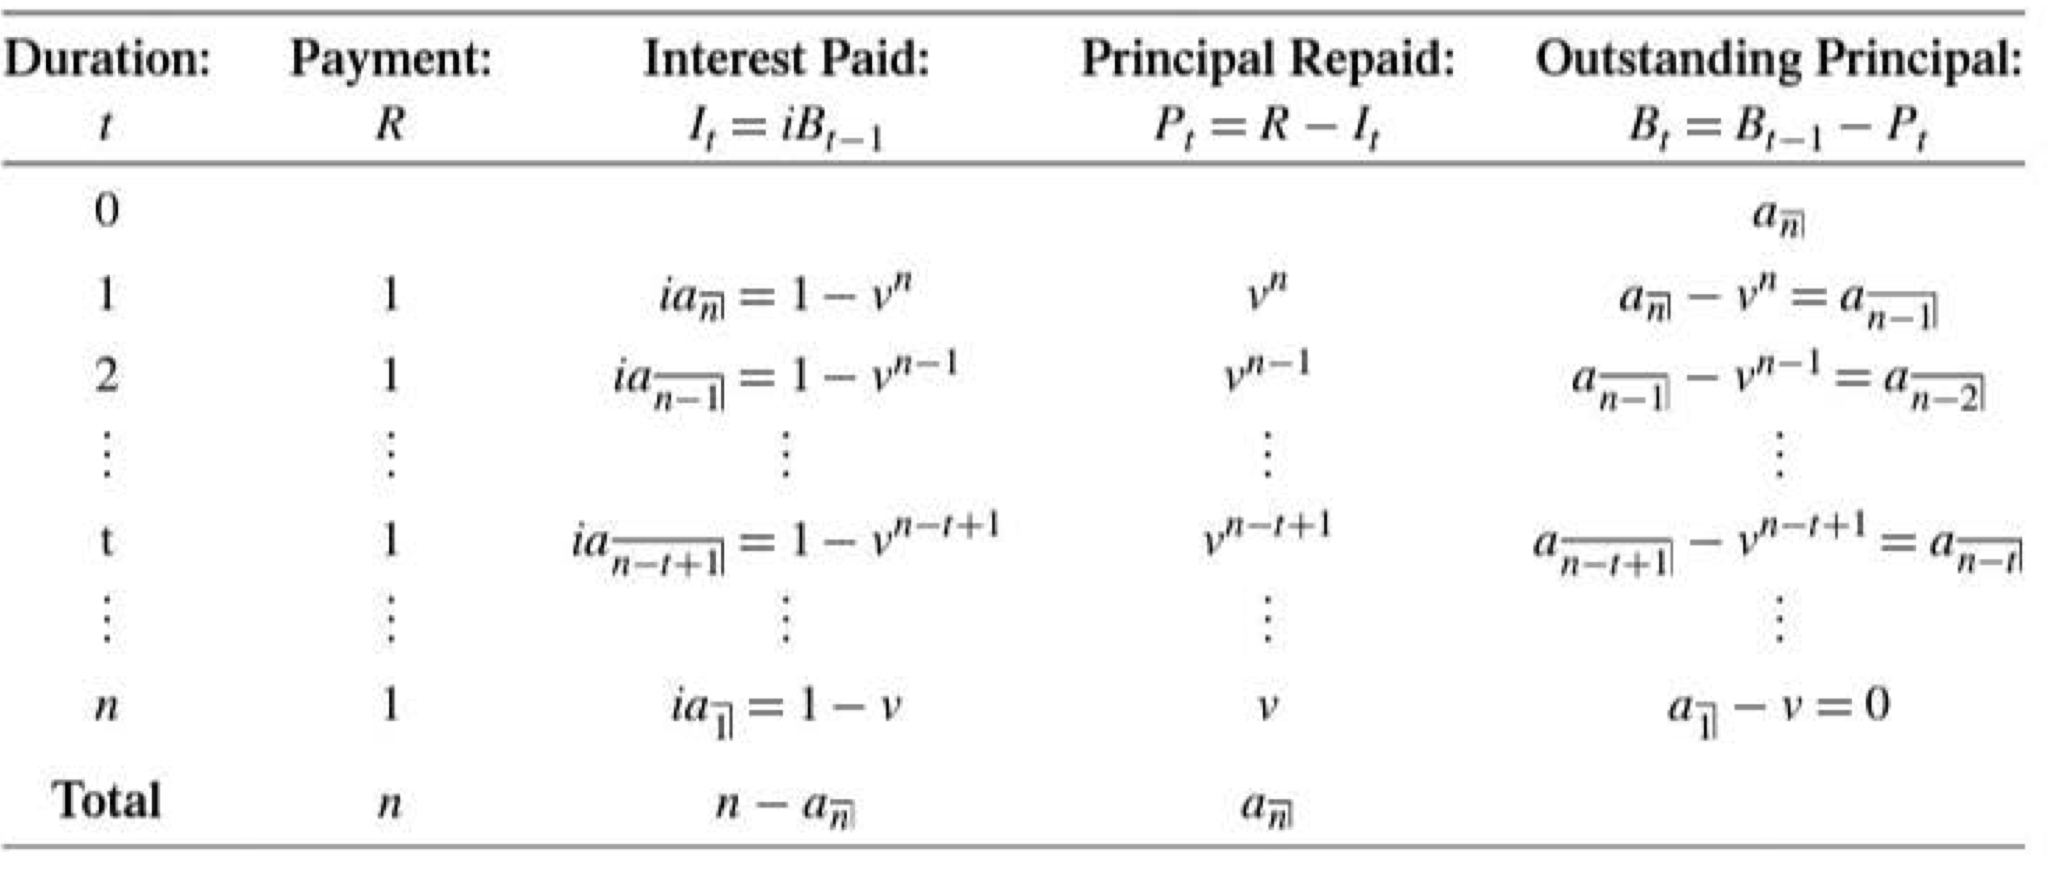
\includegraphics[scale=0.35]{img/amortization-schedule.png}
\end{center}

Which lead to these formulas for a loan of $\ax{\angln}$:
\begin{align*}
	I_{t}	&=	1 - v^{n - t + 1}	&
	P_{t}	&=	v^{n - t + 1}	&
	B_{t}	&=	\ax{\angl{n - t}}
\end{align*}

Also, we have the following interpretations for the totals:
\begin{description}
	\item[Total Interest Paid ($TI$)]	is the sum of the $n$ payments minus the original loan amount $\ax{\angln}$.
	\item[Total Principal Repaid ($TP$)]	is the original loan amount $\ax{\angln}$.
\end{description}

The amortization schedule can also be generalized for a loan of $L$, we simply multiply by a factor of $\frac{L}{\ax{\angln}}$ to cancel out the default loan of $\ax{\angln}$.\\

\paragraph{Note}	Do example at the end of the section showing 4 methods of calculating interest with the calculator \hl{(P. 324)}.
\end{CHPT_SUMM_AUTO}

\begin{CHPT_SUMM_AUTO}[label = {L.-6b}]{6b. Varying Series of Payments}
Any series of payments whose prevent value is equal to the loan amount will repay it.

Important to remember that for any loan:
\begin{itemize}
	\item	The \textbf{interest paid} is the interest rate times the previous \textbf{loan balance}.
	\item	The \textbf{principal repaid} is the loan payment minus the \textbf{interest paid}.
	\item	The new \textbf{loan balance} is the previous balance minus the \textbf{principal repaid}
\end{itemize}
\end{CHPT_SUMM_AUTO}

\begin{CHPT_SUMM_AUTO}[label = {L.-6c}]{6c. Equal Principal Repayments (A Special Case of Varying Payments)}
We can pay a \textbf{level amount of \textit{principal}} and the interest on the outstanding balance. This is different than a level payment as a level payment includes the interest paid on the outstanding balance.
\end{CHPT_SUMM_AUTO}
%
\begin{CHPT_SUMM_AUTO}[label = {L.-6d}]{6d. Final Payments (Balloon and Drop Payments)}

\end{CHPT_SUMM_AUTO}

\subsection{Notes sur les vidéos YouTube}

%\begin{YTB_SUMM}[label = {}]{}
%\begin{itemize}
%	\item	
%\end{itemize}
%\end{YTB_SUMM}
